\chapter{Preliminary Investigation into Modelling with the AIF}
\label{investigation}
To determine how capable current tools and frameworks are for capturing social argumentation, and the nuances between dialectic and eristic argumentation, a preliminary investigation was conducted. This aimed, firstly, to show how these tools and frameworks can be combined in a way that makes them fit for this particular purpose and, secondly, to determine the key strengths and weaknesses of this combination in relation to modelling social argumentation.


\section{Approach}
The AIF was determined to be the closest fit for purpose ontology for modelling argumentation on the social web, due to the goals of capturing practical, language-based argumentation, with the additional benefit of being readily extensible. Alongside the SIOC, the key elements of these ontologies have been combined to explicitly capture the social component of argumentation on the social web, while also modelling the formalised argument structure. This is achieved by linking the concept of a SIOC Post with that of an AIF Locution, treating a social web thread as a separate dialogue, or argument$_2$ and each post as an atomic unit within the dialogue (containing zero or more individual arguments$_1$). In the majority of cases, a single locution will translate to a single self-contained argument$_1$. However, a single post can contain a number of arguments$_1$ -- each with a number of premises and a single conclusion. In this situation a single L-node will link to multiple YA-nodes, as shown in Figure \ref{figure:graphs:aswo-multiple-ya}. In rare cases (often caused by constraints imposed on the length of a post by the service, such as the 140 character limit on Twitter), a user will spread the premises of a single argument across multiple posts to construct their argument$_1$. Figure \ref{figure:graphs:aswo-single-ya} shows how, in such a situation, multiple L-nodes will link to a single YA-node. If two users post identical statements, they still contribute two distinct locutions. However, they will both be linked to the same I-node(s), and therefore the same argument$_1$. In this situation, multiple YA-nodes may point to the same I-node, such as in Figure \ref{figure:graphs:aswo-repeated-argument}.


\begin{figure}
\centering
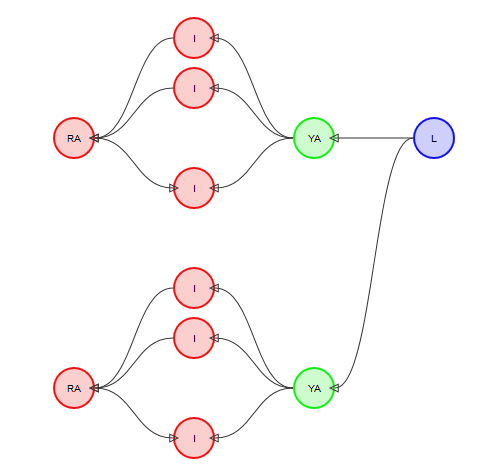
\includegraphics[scale=0.5]{./figures/graphs/aswo-multiple-ya.png}
\caption{Visualisation of one post making two distinct arguments$_1$}
\label{figure:graphs:aswo-multiple-ya}
\end{figure}


\begin{figure}
\centering
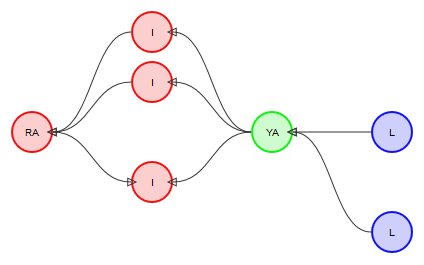
\includegraphics[scale=0.5]{./figures/graphs/aswo-single-ya.png}
\caption{Visualisation of two posts, used to construct a single argument$_1$}
\label{figure:graphs:aswo-single-ya}
\end{figure}


\begin{figure}
\centering
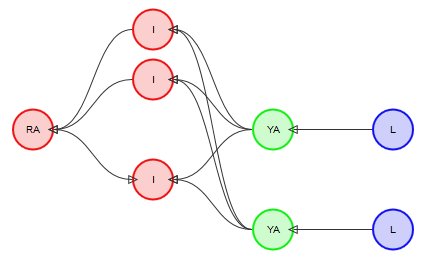
\includegraphics[scale=0.5]{./figures/graphs/aswo-repeated-argument.png}
\caption{Visualisation of two posts, repeating the same argument$_1$}
\label{figure:graphs:aswo-repeated-argument}
\end{figure}


\section{Methodology}

\subsection{Data Collection}
\label{investigation:methodology:datacollection}
A single topic of argumentation was chosen to be examined for three case studies, each representing a different social media system. To ensure the stimulation of debate, the selected topic needed to be controversial, have a large number of respondents and have been active for a long enough period of time to generate a rich and complete content. The October 2013 United States government shutdown caused by Congress's failure to agree on a budget, and the following condemnation this received from the presidency, was a suitable match for these requirements. 

This topic was then tracked across three of the social media categories identified by \citet{Kaplan2010}: Twitter, a microblogging service that allows users to publish messages of up to one-hundred and forty characters; Facebook, a social network, that allows users to create a network of ``friends'' and share text or images; and YouTube, a content creation site where users can create and upload videos, or playlists of videos.

The source of the posts themselves again needed to be both publicly available and have a large number of followers to ensure a maximally stimulated debate. As an authoritative public figure at the heart of the crisis, content from or relating to Barack Obama's social media profiles was chosen, and three posts that were broadly similar in content were selected for study. The first post, initially posted on 8th October 2013 from the White House's YouTube channel\footnote{https://www.youtube.com/watch?v=7LwoudGfug0}, is a 14m 40s video recording of Obama delivering a statement to press from the West Wing of the White House, condemning the shutdown. The post taken from Obama's official Twitter account\footnote{https://twitter.com/BarackObama/status/390288744235823104} (which is managed by a third party, Organizing for Action), dated 15th October 2013, reads: \textit{``This is unacceptable. Tell Tea Party Republicans to stop holding our economy hostage: http://OFA.BO/qNmA3Y''}. The included hyperlink leads to an Organising for Action page, which encourages users to to voice their displeasure at the shutdown by allowing them to automatically generate and send tweets. The post taken from Obama's official Facebook account\footnote{https://www.facebook.com/photo.php?fbid=10151874920756749} (also managed by Organizing for Action), also dated 15th October 2013, reads: \textit{``Tea Party Republicans in the House of Representatives forced a government shutdown, and now they're threatening an economic shutdown. This has gone on for too long. Tell them to \#EndThisNow: http://OFA.BO/ACC7qB''}.

The discussions surrounding these posts were acquired by collecting comments replying to each initial post, and those replying to subsequent posts in the discussion (taking into account only direct replies, rather than mentions within the text of the post), with the use of the public Twitter, Facebook and Youtube APIs respectively. This data was translated to an RDF triple-store using SIOC to record the data specific to the social media platform, such as which User created which Post and which Thread stores which Posts. This was used in conjunction with the DCTerms ontology, which held supplementary data such as timestamps.

\begin{table}
\centering
\caption{Metrics of total dataset collected from YouTube, Twitter and Facebook}
\label{table:results:totalstats}
\begin{tabular}{ l | r  r  r }
\textbf{Metric} & \textbf{YouTube} & \textbf{Twitter} & \textbf{Facebook} \\
\hline
Total number of posts 				& 2719 & 137 & 9494 \\

Total number of users 				& 1255 & 33 & 6224 \\

Average posts per user 				& 2.17 & 4.15 & 1.53 \\

Average words per post 				& 26.74& 15.91 & 40.12  \\

Average characters per post 		& 150.13 & 97.63 & 241.14 \\

Time between first and last posts 	& 101d 16h 19m 12s & 0d 13h 40m 48s & 90d 19h 55m 12s\\

Average time between posts			& 53m 52s & 3m 02s & 13m 47s \\

\end{tabular}
\end{table}


\subsection{Data Sampling and Annotation}
\label{method:annotation}
Because of the volume of the data produced over the course of the tracked event and the time-intensive nature of manually annotating the data, it was necessary to sample the data to a more manageable size before annotation could take place. To prevent information being lost when the dataset was scaled down, it was important to  ensure that the sampled graph maintained properties (such as diameter and average path length) similar to those of the raw data. To maintain these characteristics, ``forest fire'' sampling \citep{leskovec2005graphs, leskovec2006sampling} was used to create a sub-graph that preserved the overall structure of the parent. The algorithm for forest fire sampling is as follows:
\begin{enumerate}
\item Choose a ``forward burning probability'' $p$ -- in this instance a value of 0.7 was chosen based on the recommendation by \citet{leskovec2006sampling} for scaling down a larger graph

\item Choose a random starting node
\label{enum:forest-fire:start}

\item Add this node to the sample graph. Select $x$ nodes at random from all nodes linked to the chosen node, where $x$ is a random number geometrically distributed with mean $\frac{p}{1-p}$. If the selected node has fewer than $x$ linked nodes, select all available nodes, and return to step \ref{enum:forest-fire:start}.
\label{enum:forest-fire:recurse}

\item With each selected node, recursively repeat step \ref{enum:forest-fire:recurse} until the desired sample size has been reached. 
\end{enumerate}

Thirty posts from within the following discussion (i.e. not including the original posts) were selected using this method. This data was then manually annotated with the formal argument$_1$ information. Specifically, from each L-node, both explicit and implicit I-nodes were extracted and related together using the most appropriate S-nodes. %For example, Obama's original Twitter post (an L-node) states: \textit{``This is unacceptable. Tell Tea Party Republicans to stop holding our economy hostage: http://t.co/y8fPF8s3bG''}. From this the following I-nodes can be extracted: \textit{``The Tea Party Republicans are holding the economy hostage''}, \textit{``Holding the economy hostage is an unacceptable tactic''} and \textit{``The Tea Party Republicans should stop holding the economy hostage''}. From this, it is easy to see that the single locution contains two premises and a conclusion (which therefore need to be joined using an RA-node). This argument$_1$ can then be mapped to the specific locution by means of a YA-node.

\begin{table}
\centering
\caption{Metrics of discussions sampled from YouTube, Twitter and Facebook}
\label{table:results:samplestats}
\begin{tabular}{ l | r r r r }

\textbf{Metric} & \textbf{YouTube} & \textbf{Twitter} & \textbf{Facebook} & \textbf{All}\\
\hline
Total number of posts & 30 & 30 & 30 & 90\\

Total number of users & 23 & 12 & 30 & 65\\

Average posts per user & 1.30 & 2.50 & 1.00 & 1.38\\

Average words per post & 26.77 & 16.33 & 42.10 & 33.18\\

Average characters per post & 147.90 & 101.20 & 259.67 & 201.70\\

Time between first and last posts & 4d 0h 54m 56s & 0d 5h 13m 33s & 3d 12h 13m 18s & n/a\\

Average time between posts & 3h 20m 31s & 0h 10m 49s & 2h 54m 15s & 0h 17m 10s\\

\end{tabular}
\end{table}

\section{Results and Analysis}
\label{investigation:results}
An overview of the raw data collected from each platform is shown in Table \ref{table:results:totalstats} and the sampled data in Table \ref{table:results:samplestats}. In total, the discussion generated by the Twitter post has slightly over one-hundred and thirty replies -- in contrast, the  YouTube comments total nearly three thousand posts, and the Facebook discussion has well over nine-thousand. Each platform sees the vast majority of posts contributed soon after the initial post. However, each has a ``long tail'' of responses that gradually decrease in frequency as time goes on. The discussion on Twitter seems particularly ephemeral, with participants only contributing for a short time before moving onto other topics; while the Facebook and YouTube posts appear more ``permanent'', with users finding and contributing to them months later.

\begin{table}
\centering
\caption{Aspects of raw data from social media APIs capable of being modelled using the AIF or SIOC ontologies}
\label{table:method:features}
\begin{tabular}{ r | c | c }

\multirow{2}{*}{\textbf{Features present in social media APIs}} & \multicolumn{2}{c}{\textbf{Represented in:}}\\

 & \textbf{AIF} & \textbf{SIOC} \\
\hline
Locution (explicit content)& $\checkmark$ & $\checkmark$ \\

Illocution (premises/conclusions) & $\checkmark$ & \\

Argumentation structure (attacks/support) & $\checkmark$ & \\

Author  		& $\checkmark$ & $\checkmark$ \\

Avatar  		&  			   & $\checkmark$ \\

Replies 		& $\checkmark$ & $\checkmark$ \\

Creation Date  	& $\checkmark$ & $\checkmark$ \\

Reputation (e.g. ``Likes'')  &  &  \\

Location  &  &  \\

User ``Type'' (i.e. individual/business/etc.)  &  &  \\

Sentiment (implicit content) &  &  \\

\end{tabular}
\end{table}

In addition, when collecting this data it became apparent there was information that had no appropriate representation in either ontology, such as reputation systems (for example, the ``Likes'' used by Facebook), the sentiment of the post (for example, sarcasm, humour, abuse) or information about the type of user making the remark (whether they are an individual, a celebrity, a corporation, etc.); these omissions are shown in Table \ref{table:method:features}. These features could have substantial bearing on the perception of the argument$_2$. Consider the example of reputation systems: a retort stating \textit{``You're an idiot''} may be perceived very differently by the audience if it has no up-votes, one up-vote or one hundred thousand up-votes. Alternatively, consider a user making the argument$_1$ that \textit{``I really love using this product''}: whether the statement is made by an individual, or the company selling the product would likely influence the validity and value of the statement.

%\begin{figure}
%\begin{center}
%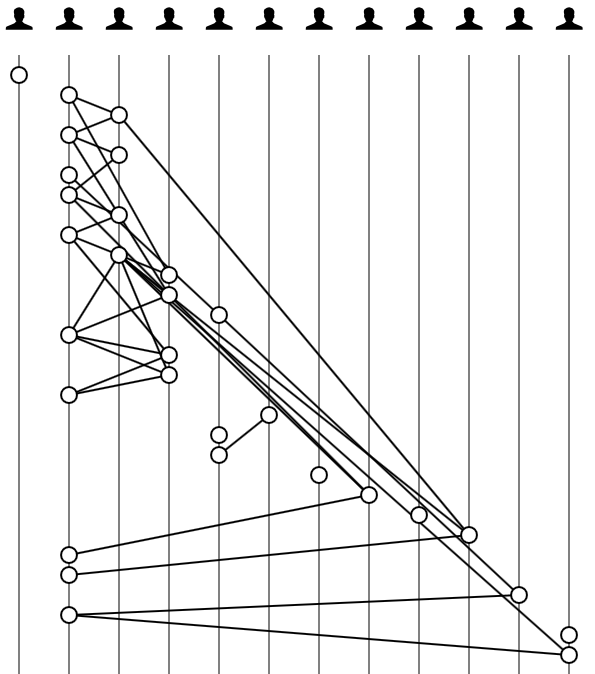
\includegraphics[scale=0.5]{./figures/lifelines_twitter.png}
%\caption{A subset of thirty Twitter replies, sampled using the forest-fire technique, visualised using Lifelines}
%\label{figure:lifelines-twitter}
%\end{center}
%\end{figure}

%\begin{figure}
%\begin{center}
%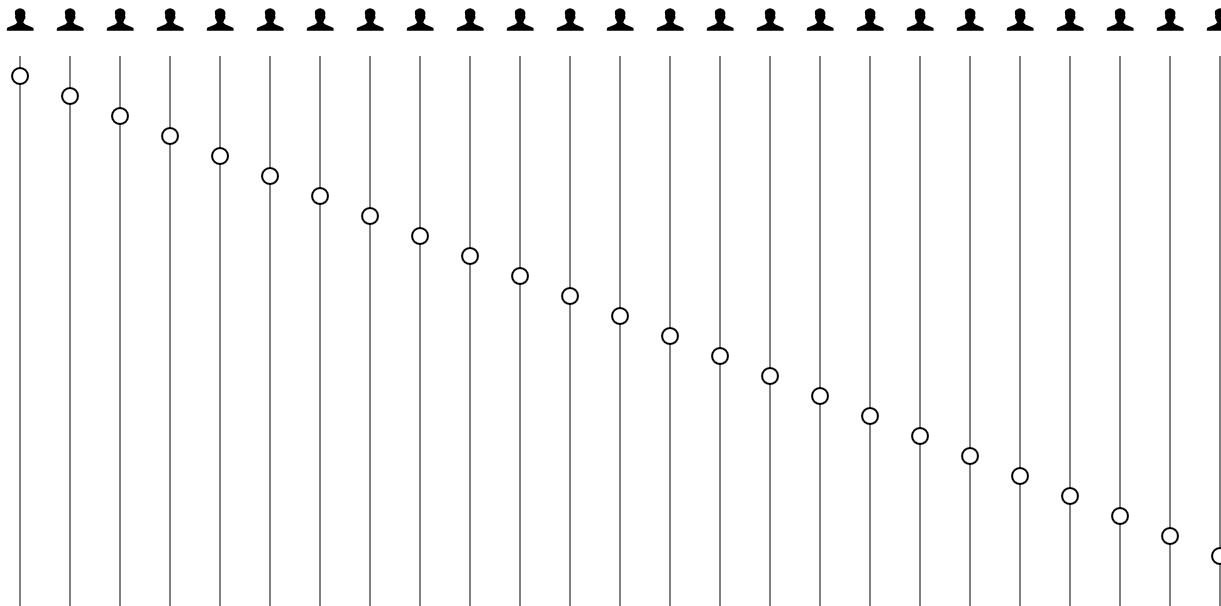
\includegraphics[scale=0.45]{./figures/lifelines_facebook.png}
%\caption{A subset of thirty Facebook comments, sampled using the forest-fire technique, visualised using Lifelines}
%\label{figure:lifelines-facebook}
%\end{center}
%\end{figure}

Table \ref{table:results:annotations} shows the statistics collected after annotating the data with premises and conclusions, represented as AIF nodes. Given this data it can be seen that Twitter is the only sample that contains Transition-nodes; that is, replies to other posts within the thread. While this may appear to suggest that the platform is used more fore debate than the others, it is possible this is down to deficiencies in the APIs of the other platforms, which often do not accurately highlight replies. It can also be observed that the debates on Twitter and Facebook have a much higher information content than that of YouTube. The resulting structures are visualised in Figure \ref{figure:speechacts}, which shows a side-by-side comparison of the three different samples.

\begin{table}
\centering
\caption{Summary of AIF nodes found in annotated discussions collected from YouTube, Twitter and Facebook}
\label{table:results:annotations}
\begin{tabular}{| l | c | c | c | c |}
\hline
\textbf{Metric} & \textbf{YouTube} & \textbf{Twitter} & \textbf{Facebook} & \textbf{Total} \\
\hline
L-nodes 			& 30	& 30 	& 30 	& 90\\
\hline
TA-nodes 			& 0		& 20 	& 0 	& 20\\
\hline
YA-nodes 			& 31	& 30	& 41 	& 102\\
\hline
I-nodes 			& 88	& 116	& 110 	& 314\\
\hline
S-nodes 			& 13	& 30    & 26 	& 69\\
\hline
L- to I-node ratio 	& 15:44	& 8:29  & 3:11	& 45:157\\
\hline
\end{tabular}
\end{table}

\begin{figure}
\centering
\begin{minipage}[b]{.30\textwidth}
  \centering
  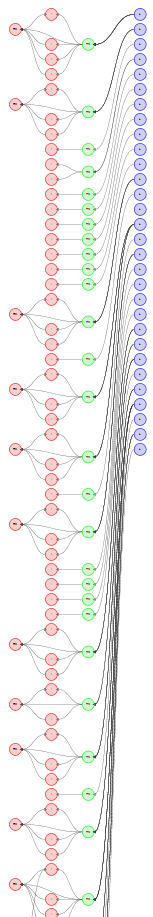
\includegraphics[scale=0.5]{./figures/speechacts/youtube.png}
\end{minipage}
\hspace{.05\textwidth}
\begin{minipage}[b]{.30\textwidth}
  \centering
  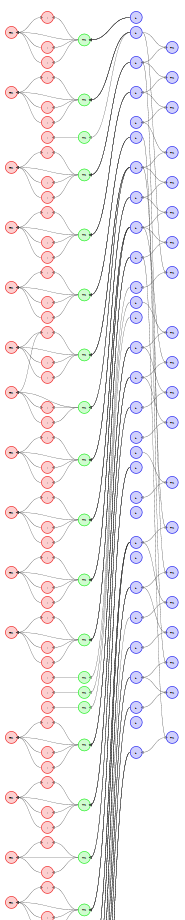
\includegraphics[scale=0.5]{./figures/speechacts/twitter.png}  
\end{minipage}
\begin{minipage}[b]{.30\textwidth}
  \centering
  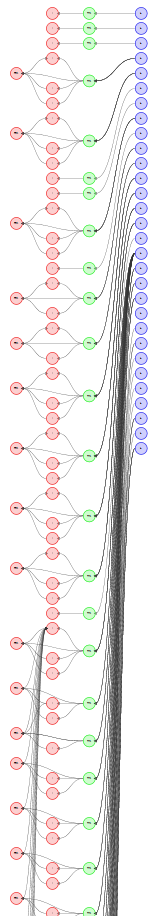
\includegraphics[scale=0.5]{./figures/speechacts/facebook.png}  
\end{minipage}

\caption{A side-by-side comparison of the emergent structures of discussions taken from YouTube (left), Twitter (centre) and Facebook (right)}
\label{figure:speechacts}
\end{figure}

On the surface, the sample of posts taken from Twitter and Facebook appear to have similar information content. However, upon manual inspection, it can be seen that this average is actually heavily skewed by one particular Facebook post that is thirteen paragraphs long and contains a total of twenty six information nodes. The argument in question is reproduced on a number of different websites, and is likely reused in full as a boilerplate ``cut and paste'' rebuttal by many users when engaging in an argument on that topic.

To highlight the overall information disparity take, for example, the tweet \textit{``@BarackObama Stop expanding government, spying on Americans and driving up the deficit.''}. This is an enthymeme -- the literally derived I-node acts as a conclusion, while the premises (that Obama is expanding government, spying on Americans and driving up the deficit  and that to do so is a bad thing) are left implicit. In turn, contrast with the posts \textit{``first''}, \textit{``wow obama''} and \textit{``lolollll i love this''} which contain very little information, either explicit or implicit. In addition, not all posts with a large amount of literal content have a comparatively large amount of information. For example, posts such as \textit{``Give DIRETIDE Give DIRETIDE Give DIRETIDE...''} (repeated upwards of fifty times in a single post) show a desire to derail the discussion by flooding it with completely irrelevant information (``Diretide'' refers to a cancelled seasonal event in the popular online game \textit{Defence of the Ancients 2}; the cancellation sparking uproar from the fanbase which led to a number of social media platforms being flooded with this message).

In addition, there are other posts that have deeper contextual meaning that would first appear. Consider, for example, ``RedScareBot''\footnote{https://twitter.com/RedScareBot}: this is an automated Twitter account that, using the avatar of Joseph McCarthy (an American politician famous for making claims at the height of the Cold War that their were numerous Soviet agents in the US government), replies to any tweet that includes phrases such as ``communism'' or ``commie'' with quips such as \textit{``Commie Chameleon''}, \textit{``Oh noes, Socialism''} or \textit{``Rise of the USSA''}. While this may seem nonsensical or a non-sequitur without context, \textit{with} context it can be viewed by the audience as a derisive or satirical retort to a knee-jerk insult, despite being posted by a machine.

There are of course limitations on the conclusions that can be drawn from a relatively small dataset when working with proverbial ``big data''. As such, these findings cannot be used to justify broad claims that state that \textit{all} arguments on a particular example of social media are structured in this way. These examples instead serve to demonstrate the important fact that different types of structures \textit{can} evolve, and provide some examples of the argumentative and rhetorical tactics people use when arguing over social media and how the conjunction of the AIF and SIOC projects (as well as any extensions made to these) can be used in attempts to map them.


\section{Summary}
\TODO{Summary}
\TODO{This shows that, currently, it is insufficient to use the AIF (and its extension) to fully model eristic argumentation, even when certain social aspects are  modelled through other ontologies such as SIOC.}